\documentclass[english,12pt]{article}
\usepackage[T1]{fontenc}
\usepackage{geometry}
\geometry{verbose,bmargin=2.5cm,lmargin=2.5cm,rmargin=2.5cm}
\usepackage[utf8]{inputenc}
\usepackage{amsmath}
\usepackage{amsfonts}
\usepackage{amssymb}
\usepackage{rotfloat}
\usepackage{wasysym}
\usepackage{graphicx}
\usepackage{natbib}
\usepackage{latexsym}
\usepackage{caption}
\usepackage{flafter}
\usepackage{babel}
\usepackage{imakeidx}
\usepackage{amssymb,amsmath}
\usepackage[table]{xcolor}
\usepackage[mathlines,displaymath]{}
\usepackage{anyfontsize}
\usepackage{verbatim}

\newcommand{\etal}{{et~al.{}}}
\newcommand{\ie}{{i.~e.{}}}
\newcommand{\eg}{{e.~g.{}}}
\newcommand{\viz}{{viz.{}}}
\newcommand{\etc}{{etc.{}}}
\newcommand{\apriori}{{a priori{}}}
\newcommand{\vv}{{vice versa{}}}
\newcommand{\cf}{{}}
\usepackage{titling}
\usepackage{color}


\date{}

\topmargin 0.0cm
\oddsidemargin 0.5cm
\evensidemargin 0.5cm
\textwidth 16cm 
\textheight 22cm

\makeindex
\begin{document}
\begin{flushleft}
\textbf{\Large {$\mathcal{ROBHOOT}$} -- An Open multilayer platform for data integration, inference and prediction}
\\
\begin{figure}
\vspace{-3 in}
\begin{center}
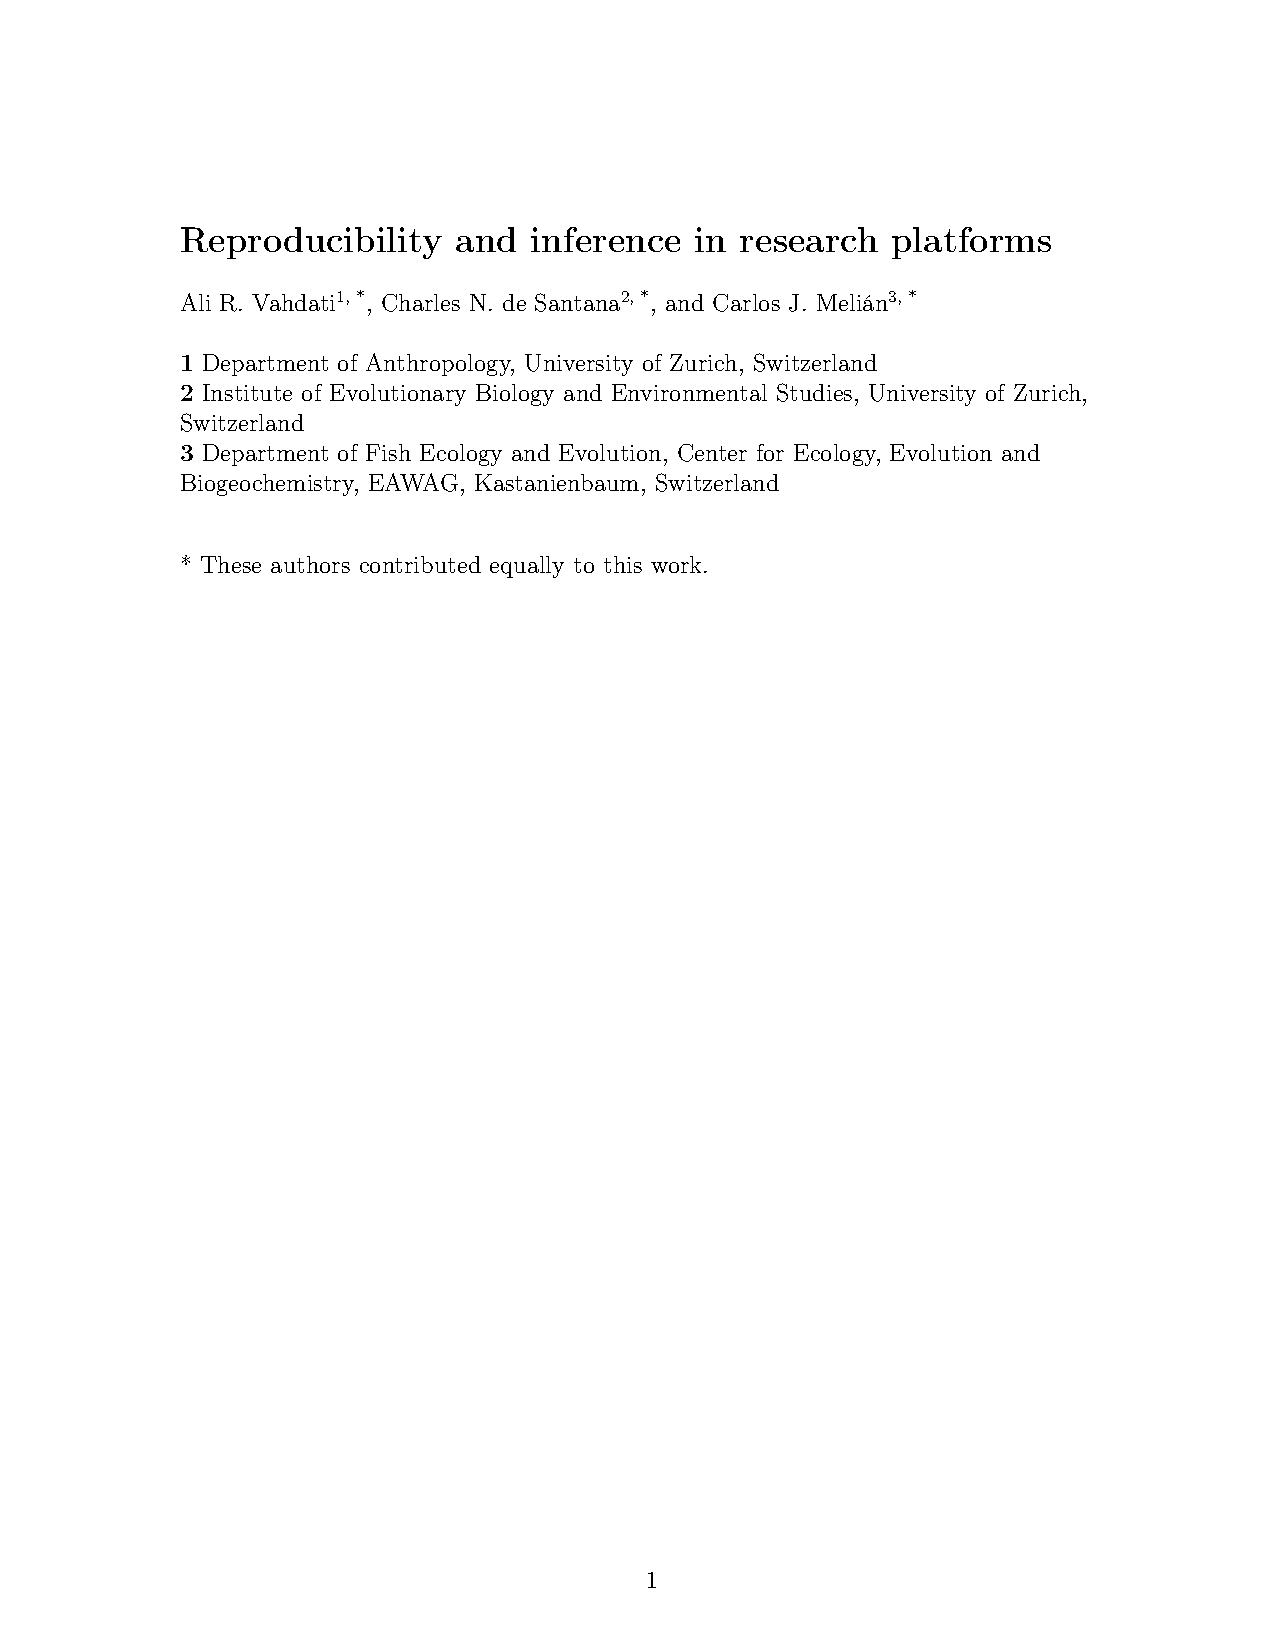
\includegraphics[scale=0.4]{robhoot.pdf}
\end{center}
\caption{Our dream icon $\mathcal{ROBHOOT}$}
\end{figure}
\end{flushleft}

\newpage


\tableofcontents
\newpage

\section{Summary}

High-resolution data coming from many sources is becoming standard in many
scientific fields. Yet, inferring insightful patterns and drivers
using integrative frameworks remains challenging in many
disciplines. Robhoot aims to develop approaches to integrate data,
statistical Learning, AI algorithms and process-based models to take
better informed decisions in research, management and investment
landscapes.
\\
Keywords: automated data integration, multilayer networks, approximate Bayesian computation, process-based inference.
\newpage


\section{Introduction}

$\mathcal{ROBHOOT}$ will be a semi-automated tool combining
access to high-resolution data from both centralized and decentralized platforms. To achieve such a combination, we aim to
develop $\mathcal{ROBHOOT}$ in two stages. The first stage will be to
develop the free-access platform to have access to high-resolution
data. The second stage will
be to run automatically ...
\\
Flowchart 1: fully connected graph using the 5 layers\\ 
Start with a simple example\\

The main five components can be described as follows: 
...summarize here the 5 layers and why
\\

\section{Data Collection (DC)}

Data access platforms from genomes to ecosystems and markets of
any kind are highly regulated. This means most interacting agents in
the market have to deal with a highly complex set of regulations
before having access to the data, algorithms and the available
strategies. Having ``easy'' access to the information in a ``perfectly
informed market'' should be simple and efficient, but unfortunately,
it is not. We aim to collect and clean data received from different sources. The
collected data can be available in CSV, database, or "real time"
(e.g. [Nakamoto Terminal](https://www.nterminal.com), [BigQuery](
https://cloud.google.com/bigquery/)). We aim to have a package in
Julia language and let the user automatically get the data in their
desired format.


\section{Complexity Reduction (CR)}

Data dimension reduction is a second step to increase performance during the next stages of analysis. 
Complexity reduction in economics and in ecology has a long tradition mostly by looking at variance-covariance matrices.
Portfolio theory in economics has a long tradition \citep{MarkowitzBook}. The theory is rooted in the concept of
efficient frontier\index{efficient frontier}. There are several packages in several languages to
calculate efficient frontiers\footnote{\url{http://www.quantcode.com/}}$^{,}$\footnote{\url{https://github.com/JuliaQuant/PortfolioModels.jl}}$^{,}$\footnote{\url{https://www.wikinvest.com/account/portfolio/register}}$^{,}$\footnote{\url{https://d1so5k0levrfcn.cloudfront.net/SigFig\%20Investment\%20Methodology.pdf}}. Most maths underlying portfoliio theory\index{portfolio theory} are
based in matrix correlation patterns\index{matrix correlation patterns}. In ecology, portfolio concept has also been used to predict the number of coexisting species in landscapes with highly fluctuating environments\footnote{Check references}.

Many fields aim at predicting fluctuations of several time series at local and regional scales. The better the predictions are the better we know the ecosystem. Unfortunately,
  it is not easy to predict time series of a large number of
  interacting (ideally independent) variables. Given we can not predict most of the
  ideas' trends, we should build a minimum understanding on how to
  investigate ideas and build a diversified portfolio with a balance
  between risk and reward. Basic questions will always remain when
  discussing about predicting the future and diversifying
  portfolios. For example, in a complex ecosystem, which is the best
  strategy under complete ignorance? And under complete information?
  Should we invest in ideas following a random walk \index{random walk}? Should
  we produce a portfolio with neutral risk \index{neutral risk}?
  \footnote{\url{https://en.wikipedia.org/wiki/A$_$Random$_$Walk$_$Down$_$Wall$_$Street}}. Given the basic maths underlying complexity reduction, which are the
algorithms and models out there? Which one perform the best? Which is
the mixed of models to minimize data complexity?
\\

\section{Pattern Inference (PI)}

Outline classical variance-covariance matrices, AI
algorithms and process-based methods.

\section{Model Validation (MV)}

Describe briefly Bayesian Inference, Approximate Bayesian computation, AIC and BIC model comparison methods.


\newpage
\section{Acknowledgments}


\newpage
\bibliographystyle{evolution}
\bibliography{ref}

\newpage

\section{Tables}


\newpage

\section{Figures}

%Figure 1: Flowchart 1 5 fully connected layers and a example

%Figure 2: ROBHOT: Steps to develop ROBHOT
%\begin{figure}
%\vspace{-1 in}
%\begin{center}
%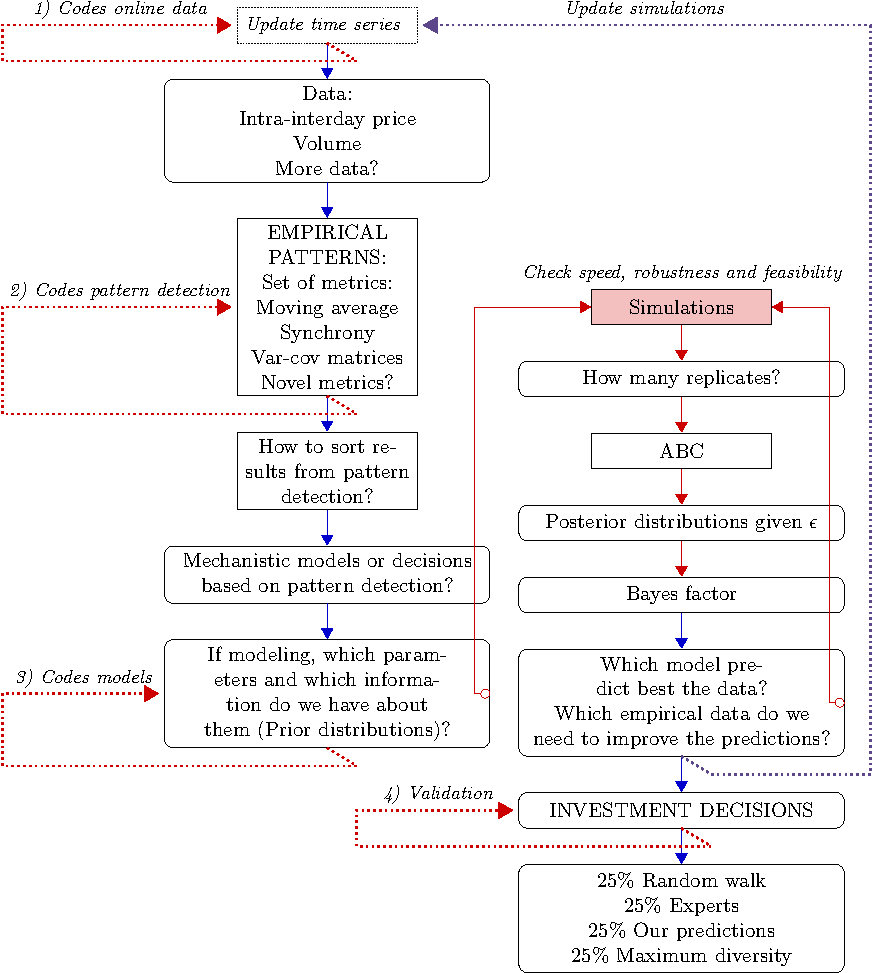
\includegraphics[scale=0.8]{EasyFlowChart.pdf}
%\end{center}
%\caption{Flow chart summarizing the steps to develop $\mathcal{ROBHOOT}$}
%\label{}
%\end{figure}
%\newpage

%Figure 3: ROBHOT: Steps to develop ROBHOT
%\begin{figure}
%\vspace{-1 in}
%\begin{center}
%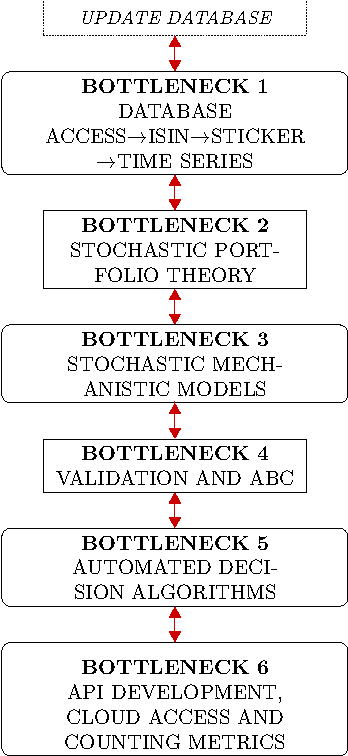
\includegraphics[scale=1.25]{EasyFlowChartBottlenecks.pdf}
%\end{center}
%\caption{Bottlenecks to overcome to develop $\mathcal{ROBHOOT}$}
%\end{figure}
%\newpage


\printindex
\end{document}
